\title{Requirements Analysis Report}
\author{
	\textbf{Group 7} \\ \\
	Harry Stevenson \\
	Stephen Lynn \\
	David Todd \\
	Liam Joy \\
	Thomas Gak Deluen
}

\documentclass[11pt, oneside, a4paper]{article}
\usepackage[table, xcdraw]{xcolor}
\usepackage{graphicx}
\usepackage[margin=1in]{geometry}
\bibliographystyle{plain}

\begin{document}

\clearpage
\maketitle
\thispagestyle{empty}

\newpage
\setcounter{page}{1}

\section{Abstract}
This document is for the use of the stakeholders (Deutsche Bank) and the assessor (Professor Stephen Jarvis),
along with the software developers, it will outline the requirements of the software to be developed for
these stakeholders, for discussion in a meeting on Friday 10th February.

\section{Introduction}
We have been given a largely simplified version of the FTSE 100 stock market to identify anomalous data, we
acknowlegde that in a real-life situation, the data would be much more complex. Therefore, our system should
have the ability to be adapted to identify anomalous data in multiple different situations.\\\\
The task set is to produce software to help the stakeholders identify and flag anomalous trading patterns
on the London Stock Exchange for stocks within the FTSE 100. This is to provide an `early warning' system
to alert the bank to rapid market changes that would be too fast to spot manually. Without this, the
stakeholders would be left vulnerable and less aware to the events causing major fluctuations within the
stock market and potentially catch rogue traders, looking to exploit the market using novel, unknown techniques.
The identification of such events must be done in a live data environment and the software must be capable of
coping with the fast-moving nature of the dataset required, reducing human intervention, thus reducing the workload
of analysts to a manageable level allows them to spend less time searching for these aberrations and more time
responding to them.

\section{User Requirements}
\subsection{Functional Requirements}
The system must:
\begin{itemize}
	\item \textbf{C:} Learn characteristics of stocks in the FTSE 100 such as the fluctuation amount, average, minimum and maximum volumes and prices of individual stocks
	\begin{itemize}
		\item \textbf{D:} Use a machine learning algorithm to update the characteristics of stocks based on the statistical analysis
	\end{itemize}
	\item \textbf{C:} Analyse the incoming data to detect if there is an anomalous trading pattern occurring
	\begin{itemize}
		\item \textbf{D:} Through statistical analysis, find a distribution to fit data which will allow entries that are far away from an average value can be categorised as anomalous
		\item \textbf{D:} Flag as anomalous when the probability of a volume or price value occurring are less than a prescribed percentage
	\end{itemize}
	\item \textbf{C:} Send an alert to notify the analysts examining the data when an anomalous trading pattern occurs
	\begin{itemize}
		\item \textbf{D:} The alert should be created in the backend as a result of the analysis of the data before being fed into the frontend and displayed on the user interface
	\end{itemize}
	\item \textbf{C:} When an alert is received, the user should be able to obtain the relevant data to ‘drill down’ into the data and allow them to perform root cause analysis
	\begin{itemize}
		\item \textbf{D:} When the user clicks on an alert, it should retrieve data for that particular stock from the database and display on screen such that the user can analyse this
	\end{itemize}
	\item \textbf{C:} Be able to analyse both a live feed and static market data
	\begin{itemize}
		\item \textbf{D:} Connect to server on port 80 and receive and parse the incoming ascii data
		\item \textbf{D:} allow the user to upload a static csv file, be able to open this, parse and analyse the data included in it, running in the background while still collecting live data
		\item \textbf{D:} A sample of the data that is
	  required to be analysed can be seen in figure \ref{SampleData}, this includes the timing of the trade, the relevant
	  buyer and seller, the price, volume, stock ticker symbol, sector as well as the bid and ask prices. In this also, is the
	  market on which the trade was made, however this is irrelevant as this will always be the London Stock Exchange GBX.
	  \begin{figure}[h]
		\centering
  	  		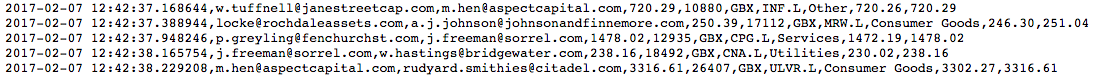
\includegraphics[width=350px]{SampleData.png}
		\caption{Data sample taken from the live data feed}
	  	\label{SampleData}
	  \end{figure}
	\end{itemize}
	\item \textbf{C:} Be able to cope with the connection and reconnection of the server from which it receives the live data
	\begin{itemize}
		\item \textbf{D:} When the server refreshes at 12am, the software must disconnect safely, retaining all data before reconnecting at 1am when the server resumes publishing data
	\end{itemize}
\end{itemize}

\subsection{Non-Functional Requirements}
The system should also:
\begin{itemize}
	\item \textbf{C:} Remain responsive whilst being able to process the large dataset required such that delays are kept to a minimum
	\begin{itemize}
		\item \textbf{D:} The delay between a rogue trading pattern occurring and it being detected and flagged on screen for the user should not exceed 5 seconds such that the anomalous data can be caught and the information used effectively
	\end{itemize}
	\item \textbf{C:} Have a simple, effective display of the current system status, suggesting if action is needed to be taken or not
	\begin{itemize}
		\item \textbf{D:} The home page for the system should display clearly if there are any anomalous trading patterns that have not been analysed and actioned by the user
		\item \textbf{D:} Data already in possession of the analysts utilising this system need not be replicated in full, only to be retrieved in showing the user where the anomalous trade may have occurred
	\end{itemize}
	\item \textbf{C:} Be suitable for non-technical users
	\begin{itemize}
		\item \textbf{D:} Use sliders and similar methods for the user to modify the algorithm used to analyse the data, along with levels of strictness rather than numerical values
	\end{itemize}
	\item \textbf{C:} Have a consistent, strong user interface to the design of the system
	\begin{itemize}
		\item \textbf{D:} Use similar themes and styling (e.g. fonts, colours etc.)
		\item \textbf{D:} Do not use clashing colours, such that text is clear to read
	\end{itemize}
	\item \textbf{C:} Display data in an appropriate way such that it is easy to extract data required to understand situation
	\begin{itemize}
		\item \textbf{D:} Display data on stock prices and volumes in graphs and tables, there should not be more than 2 visualisations of the data on the screen at a time such that the data can be displayed at a reasonable size and such the data visualisation is not excessive
	\end{itemize}
	\item \textbf{C:} Be validated using appropriate methods
	\begin{itemize}
		\item \textbf{D:} Before handing over to customer, perform rigorous testing (as laid out in the planning \& design document) to ensure responsiveness, smooth running and the success of it identifying anomalous trade patterns. This will complement such unit tests that will be made throughout the design and implementation process
	\end{itemize}
\end{itemize}

\subsection{Requirements Out of Scope}
The system should not be concerned with:
\begin{itemize}
	\item \textbf{C:} Connection to any external data feeds
	\begin{itemize}
		\item \textbf{D:} apart from the data feed on cs261.dcs.warwick.ac.uk
	\end{itemize}
	\item \textbf{C/D:} Support of multiple users or a form of login system
	\item \textbf{C/D:} Requirement of any form of security measures
	\item \textbf{C/D:} Being able to integrate with existing Deutsche Bank systems
	\item \textbf{C/D:} Should not include any Deutsche Bank branding
\end{itemize}

\subsection{Stretch Goals}
In addition to these mandatory, primary requirements, the software may also:
\begin{itemize}
	\item \textbf{C:} Use data collected to provide short-term future price predictions
	\begin{itemize}
		\item \textbf{D:} Use the machine learning algorithm to extrapolate the current trend to provide a range in which the price may be in the short-term
		\item \textbf{D:} Only provide a prediction for the next 1 hour, as this would provide an accurate prediction, rather than a vague long-term prediction
		\item \textbf{Priority:} High - This is a feasible and useful feature to add to the application, providing useful data to both traders and analysts. The period for which the prediction is valid is important because in such a high precision, fast moving industry accuracy is key and many decisions must be made for the immediate future
	\end{itemize}
	\item \textbf{C:} Cope with the manipulation of whole sectors or selected groups in the market
	\begin{itemize}
		\item \textbf{D:} For each sector as seen in the data stream, keep data on the sector, similar to that data kept on each stock
		\item \textbf{Priority:} Medium - This feature would allow the system to detect trader’s attempts to stay under the radar by performing illegal trading in stocks of the same sector as opposed to just the one stock. It is also feasible as it is using similar statistical analysis on a larger dataset as it will contain a group of shares
	\end{itemize}
	\item \textbf{C:} Allow the user to adapt the machine learning algorithm performing the statistical analysis
	\begin{itemize}
		\item \textbf{D:} Give the user sliders and similar methods to select a level of strictness, to determine how extreme values should be to be flagged by the algorithm
		\item \textbf{Priority:} Low - Although this may be a useful feature for advanced users, it would be difficult to implementdue to the users not being machine learning experts and without full understanding of the underlying statistical analysis the levels to which the algorithm could be manually changed by the user would be difficult to quantify.
	\end{itemize}
	\item \textbf{C:} Automatically organise trading patterns into categories of anomalies
	\begin{itemize}
		\item \textbf{D:} When a trade is flagged up as anomalous, flag with the reason it has been flagged and name of the trading pattern associated with this behaviour
		\item \textbf{Priority:} Low - Our task is to find anomalous trading patterns that are novel and unknown techniques therefore the categorisation of this anomalous data is infeasible due to some anomalous data not falling into the known categories, but should nevertheless, still be flagged up as anomalous
	\end{itemize}
\end{itemize}

\section{Group Management}
Through a democratic vote taken from within the group discussions, it has been decided that Thomas will take on the role of
Project Manager, Liam will be the Business Analyst in contact with the customer, the Software Architect to outline the system
will be Harry, Stephen will design the look and feel of the system and David will be the Software Tester. Everyone in the group
will also be Software Developers as we endeavour to create a professional system before the deadline. Thomas shall work alongside
Stephen to create the frontend of the application, whilst still overseeing the work of Harry, David and Liam on the backend. \\\\
The whole group will meet at least once a week in the already discussed available timeslots between 10am and 12am on Mondays, Tuesdays,
Wednesdays or Fridays, although additional meetings may occur with necessary group members as required. All major decisions shall
be taken as a group vote, with the project manager's decision counting as final in the case of any tied votes, however, all decisions
involving the frontend or backend team only, will be taken from within the relevant team, including the project manager, such that it
allows consistency throughout the application.\\\\
The planning and design of the application will be done in the teams prescribed above, with both teams informing each other throughout
the process to ensure the feasibility and consistency of the application.

\newpage
\begin{thebibliography}

	\item Investopedia {\em Bear Raid} \\
	http://www.investopedia.com/terms/b/bearraid.asp \\
	Date Accessed: 07/02/2017
	\item Treanor, Jill {\em `Fat finger trade' suspected of causing sudden FTSE fall} \\
	https://www.theguardian.com/business/2015/sep/18/fat-finger-trade-suspected-ftse-100-fall \\
	Date Accessed: 07/02/2017
	\item US Securities and Exchange Commission {\em ``Pump-and-Dumps'' and Market Manipulations} \\
	https://www.sec.gov/answers/pumpdump.htm \\
	Date Accessed: 07/02/2017
\end{thebibliography}

\newpage
\appendix
\section{Questions}
\textbf{Q: Should the user be able to visually see the data parsed and in what format should it be displayed?}\\
\textbf{A:} There is no specific format mandated by DB, however good data visualisation is always important when a user needs to
understand and respond to information quickly.\\
Traders manage portfolios containing hundreds of stocks and must respond quickly to events affecting any one of them. The system
needs to make a user aware something has happened, but also give them with enough information to decide how to respond. The
challenge here is to provide enough information for the trader to make a purchasing decision quickly. \\\\
\textbf{Result:} We will not display a list of all the trade data on the screen, only when an alert is generated will the
relevant data be retrieved from the database and displayed. \\\\
\textbf{Q: Should we allow the user to manually adapt any characteristics learned by the machine learning algorithm?}\\
\textbf{A:} If you do choose to allow the user this level of control, you should be aware that the users are non-technical, meaning
they are not familiar with machine learning techniques. You should be careful to expose this functionality in a way that users can understand. \\\\
\textbf{Result:} If we choose to implement this stretch goal, then we will employ sliders and levels of strictness in the statistical
analysis, therefore giving users the ability to alter the algorithm to their needs, but also making this feature accessible to non
technical users. \\\\
\textbf{Q: As required by the specification, our software will be able to take data from a static file. However, does this imply
that the user can at any point upload a file to the software using some means of upload implemented by us?}\\
\textbf{A:} There will never be a case where a user needs to be responding to alerts from static and dynamic data simultaneously.
However, there will be times when a user will have to upload a file to your software. \\\\
\textbf{Result:} There will be separate areas of our system for the analysis of live data and the upload and analysis of other csv files,
therefore allowing both features to be implemented, but allowing a csv file to be uploaded and analysed without affecting performance of the live
data analysis. \\\\
\textbf{Q: How long is an appropriate time frame to predict future data?}\\
\textbf{A:} Your prediction horizon should be as long as your model is accurate for, and no longer. It is important to note here that `prediction'
does not mean you have to specify an exact price at an exact time in the future. It is more important to show the overall trend in the data.
A model which can provide accurate projections for the next hour or more would be considered very valuable.\\\\
\textbf{Result:} As stated in the report above, if we implement this stretch goal, we will make short-term predictions for the upcomming hour, to
ensure accuracy, but also usefulness of the predictions. The predictions made will also be given as a range of possible price values, the closer
the time in the future the prediction is, the smaller the range of possible values.

\end{document}
